\renewcommand{\tool}{WASM-MUTATE\xspace}
\msection{\tool: Fast and Effective Binary for WebAssembly}

In this section, we introduce our third technical contribution, \tool \cite{wasmmutate}, a tool that generates functionally equivalent variants of a WebAssembly binary input. 
Leveraging rewriting rules and e-graphs \cite{e-graph} for diversification space traversals, \tool synthesizes program variants by transforming parts of the original binary. 
In \autoref{fig:approach_landscape}, we highlight \tool as the blue squared tooling for a visual representation.

\begin{figure*}[h!]
    \centering
    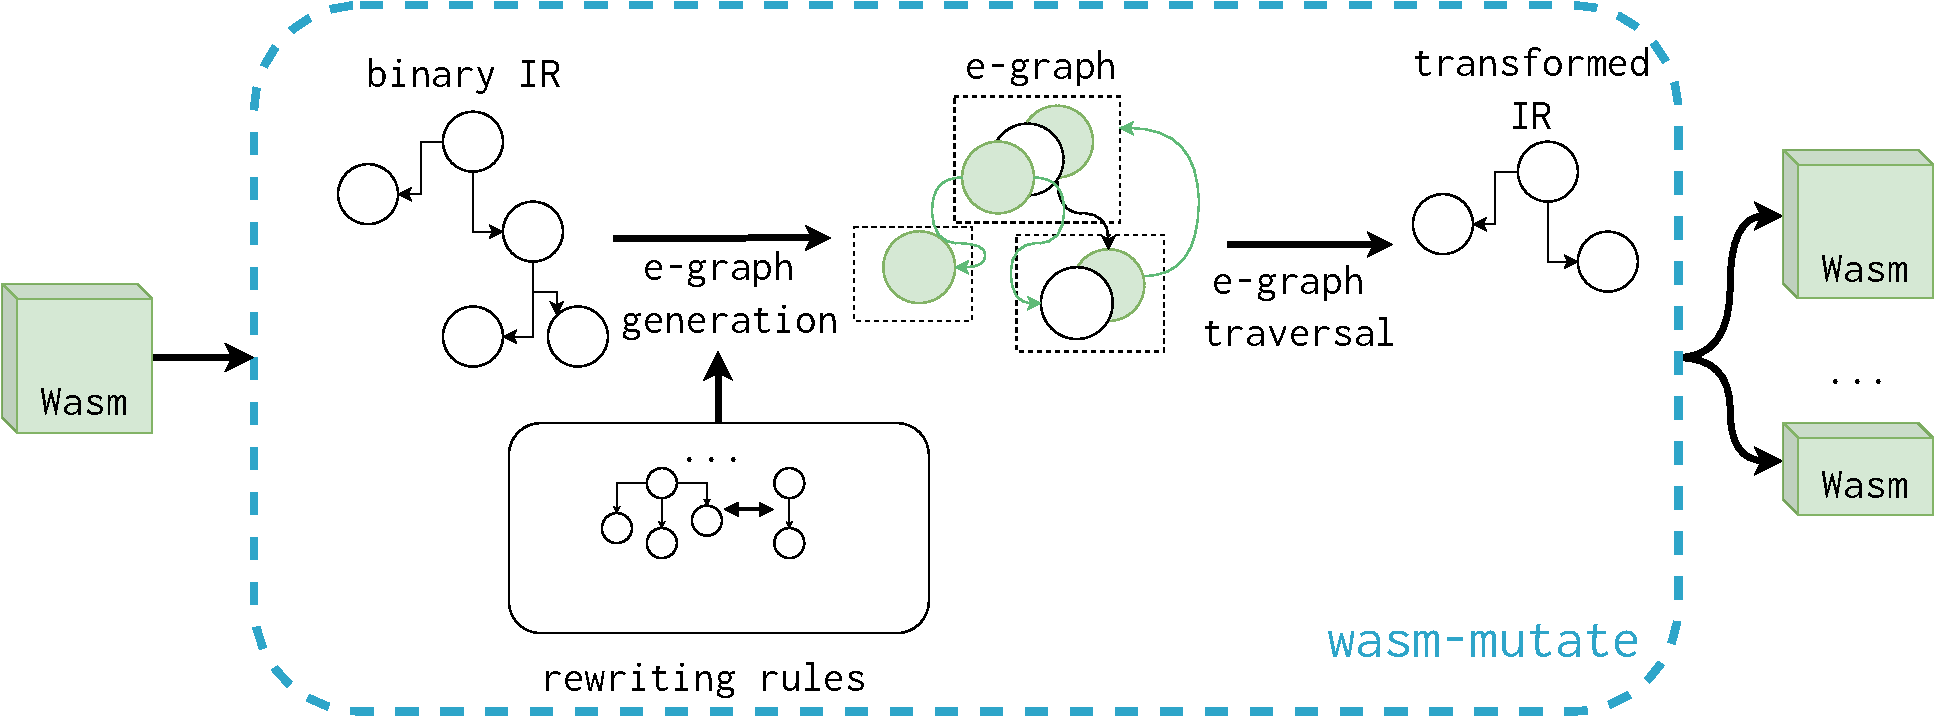
\includegraphics[width=0.9\linewidth]{diagrams/wasm_mutate.workflow.pdf}
    \caption{ \tool high-level architecture.  It generates semantically equivalent variants from a given WebAssembly binary input. 
    Its central approach involves synthesizing these variants by substituting parts of the original binary using rewriting rules, boosted by diversification space traversals using e-graphs.}
  \label{fig:wasm-mutate}
\end{figure*}


\autoref{fig:wasm-mutate} illustrates the workflow of \tool, which initiates with a WebAssembly binary as its input. 
The first step involves parsing this binary to create suitable abstractions, e.g. an intermediate representation.
Subsequently, \tool utilizes predefined rewriting rules to construct an e-graph for the initial program, encapsulating all potential equivalent codes derived from the rewriting rules. 
Then, pieces of the original program are randomly substituted by the result of random e-graph traversals, resulting in a variant that maintains functional equivalence to the original binary. 
This assurance of semantic preservation is rooted in the inherent properties of the individual rewrite rules employed.



\msubsection{WebAssembly Rewriting Rules}
\tool incorporates a total of 135 rewriting rules, organized into categories referred to as meta-rules. 
The rewriting rules are conceived based on the seminal work of Sasnauskas et al. \cite{2017arXiv171104422S}, extended to include a predicate to enforce the conditions for replacement. 
Each rule is articulated as a tuple, represented as \texttt{(LHS, RHS, Cond)}, where: \texttt{LHS} identifies the segment of code targeted for replacement, \texttt{RHS} outlines the functionally equivalent substitute, and \texttt{Cond} defines the circumstances permitting the replacements.
For example, in the case of \Wasm binaries, the \texttt{Cond} predicate ensures that the replacement does not violate the type constraints. 
The following text details the seven meta-rules utilized in \tool.


\wrule{Add type:}
\tool implements two rewrite rules for the Type Section of the input \Wasm program.
These rewriting rules create random function signatures, varying both, the number of parameters and the count of results. 
It ensures the consistency of the index of already defined types, even after the introduction of a new type.
The following listing illustrates how WASM-MUTATE adds a new type definition based on this meta-rule. 

\begin{minipage}{0.9\linewidth}
  
{\footnotesize
\lstdefinestyle{watcode}{
  numbers=none,
  stepnumber=1,
  numbersep=10pt,
  tabsize=4,
  showspaces=false,
  breaklines=true, 
  showstringspaces=false,
    moredelim=**[is][{\btHL[fill=weborange!40]}]{`}{`},
    moredelim=**[is][{\btHL[fill=celadon!40]}]{!}{!},
    moredelim=**[is][{\btHL[fill=frenchplum!40]}]{bb}{bb},
    moredelim=**[is][{\btHL[fill=eminence!40]}]{bc}{bc}
}

\lstset{
        language=ttt,
        style=watcode,
        basicstyle=\footnotesize\ttfamily,
        columns=fullflexible,
        breaklines=true}
\begin{lstlisting}[numbers=none]{Name}
LHS (module
  (type (;0;) (func (param i32) (result i64)))
        \end{lstlisting}  
\hrulefill

\begin{lstlisting}[numbers=none]{Name}
RHS (module
  (type (;0;) (func (param i32) (result i64)))
!+ (type (;0;) (func (param i64) (result i32 i64)))!
        \end{lstlisting}   
}
\vspace{2mm}
\end{minipage}

\wrule{Add function:} 
%In a \wasm binary, the function and code sections contain the function declarations and their respective code bodies. 
\tool adds new random functions by mutating the code, type, and function sections. 
This process begins with the creation of a random type signature, followed by the formulation of a random function body that simply returns the default value corresponding to the result type. 
An illustration of this transformation is provided in the subsequent example.

\begin{minipage}{0.9\linewidth} 
    
\lstdefinestyle{watcode}{
    numbers=none,
    stepnumber=1,
    numbersep=10pt,
    tabsize=4,
    showspaces=false,
    breaklines=true, 
    showstringspaces=false,
      moredelim=**[is][{\btHL[fill=black!10]}]{`}{`},
      moredelim=**[is][{\btHL[fill=celadon!40]}]{!}{!}
  }
  
  {
  \captionsetup{width=\linewidth}
  \noindent\begin{minipage}[b]{\linewidth}
      \lstset{
          language=ttt,
          style=watcode,
          basicstyle=\footnotesize\ttfamily,
          columns=fullflexible,
          breaklines=true}
          \begin{lstlisting}[]{Name}
   LHS (module
      (type (;0;) (func (param i32 f32) (result i64)))
          \end{lstlisting}
          %\vspace{0.2cm}
     \end{minipage}
     
  \noindent\hrulefill
  
  \noindent\begin{minipage}[b]{\linewidth}
      \lstset{
          language=ttt,
          style=watcode,
          basicstyle=\footnotesize\ttfamily,
          columns=fullflexible,
          breaklines=true}
          \begin{lstlisting}[]{Name}
   RHS (module
      (type (;0;) (func (param T) (result t)))
      (func (;0;) (type 0) (param T) (result t)
         t.const 0) 
          \end{lstlisting}
          %\vspace{0.2cm}
     \end{minipage}
     
  }
  
\end{minipage}

\wrule{Debloat:} \tool randomly eliminates dead parts of the input \wasm program, targeting specific elements such as \emph{functions, types, custom sections, imports, tables, memories, globals, data segments, and elements} that are verifiably unused. 
For instance, the removal of a memory declaration needs the absence of any memory access operations within the binary code. 
\tool incorporates distinct mutators for each element type to facilitate this process.
The following example showcases a function removal using this meta-rule.



\begin{minipage}{0.9\linewidth} 

\lstdefinestyle{watcode}{
  numbers=none,
  stepnumber=1,
  numbersep=10pt,
  tabsize=4,
  showspaces=false,
  breaklines=true, 
  showstringspaces=false,
    moredelim=**[is][{\btHL[fill=weborange!40]}]{`}{`},
    moredelim=**[is][{\btHL[fill=celadon!40]}]{!}{!}
}

{
    \lstset{
        language=ttt,
        style=watcode,
        basicstyle=\footnotesize\ttfamily,
        columns=fullflexible,
        breaklines=true}
         
\vspace{8mm}
        \begin{lstlisting}[]{Name}
LHS (module (type (func)))
        \end{lstlisting}
\noindent\hrulefill
    \lstset{
        language=ttt,
        style=watcode,
        basicstyle=\footnotesize\ttfamily,
        columns=fullflexible,
        breaklines=true}
        \begin{lstlisting}[numbers=none]{Name}
RHS `- (module (import "" "" (func)))`
        \end{lstlisting}

\lstset{
        language=ttt,
        style=watcode,
        basicstyle=\footnotesize\ttfamily,
        columns=fullflexible,
        breaklines=true}
        \begin{lstlisting}[numbers=none]{Name}
Cond The removed function is not called, it is not exported, and it is not in the binary _table.
        \end{lstlisting}
}
\end{minipage}


\wrule{Edit custom sections:} \tool randomly changes either the content or the name of the custom section, a process illustrated in the subsequent example.

\begin{minipage}{0.9\linewidth} 

\lstdefinestyle{watcode}{
  numbers=none,
  stepnumber=1,
  numbersep=10pt,
  tabsize=4,
  showspaces=false,
  breaklines=true, 
  showstringspaces=false,
    moredelim=**[is][{\btHL[fill=weborange!40]}]{`}{`},
    moredelim=**[is][{\btHL[fill=celadon!40]}]{!}{!}
}

{
    \lstset{
        language=ttt,
                        style=watcode,
        basicstyle=\footnotesize\ttfamily,
                        columns=fullflexible,
                        breaklines=true}
        
        \begin{lstlisting}[]{Name}
LHS (module
...
    `-    (@custom "CS42" "zzz..."`
        \end{lstlisting}
\noindent\hrulefill
        
{
    \lstset{
        language=ttt,
                        style=watcode,
        basicstyle=\footnotesize\ttfamily,
                        columns=fullflexible,
                        breaklines=true}
        
        \begin{lstlisting}[]{Name}
RHS (module
...
    !+    (@custom "CS42" "xxx...")!
        \end{lstlisting}
}
}
\end{minipage}
        


\wrule{If swapping:} In \Wasm, the if-construction is a compound of two paths: the consequence and the alternative. 
The determination of which execution path to follow depends on the branching condition evaluated just before the \texttt{if} instruction. 
Specifically, a value greater than \texttt{0} at the top of the execution stack triggers the execution of the consequence code, while any other outcome initiates the alternative code.
The \emph{if swapping} rewriting rule interchanges the consequence and alternative codes within the if-construction, effectively reversing the original paths defined by the condition.



To facilitate the swapping of an if-construction in \Wasm, \tool introduces a negation of the value situated at the top of the stack immediately preceding the \texttt{if} instruction. 
The methodology behind this rewriting is demonstrated in the following example.

\begin{minipage}{0.9\linewidth} 

\lstdefinestyle{watcode}{
  numbers=none,
  stepnumber=1,
  numbersep=10pt,
  tabsize=4,
  showspaces=false,
  breaklines=true, 
  showstringspaces=false,
    moredelim=**[is][{\btHL[fill=weborange!40]}]{`}{`},
    moredelim=**[is][{\btHL[fill=celadon!40]}]{!}{!},
    moredelim=**[is][{\btHL[fill=frenchplum!40]}]{bb}{bb},
    moredelim=**[is][{\btHL[fill=eminence!40]}]{bc}{bc}
}

{
    \lstset{
        language=ttt,
                        style=watcode,
        basicstyle=\footnotesize\ttfamily,
                        columns=fullflexible,
                        breaklines=true}
        
        \begin{lstlisting}[]{Name}
LHS (module
    (func ...) (
bb condition C bb
        (if bb A bb  else bb  B bb end)
    )
)
        \end{lstlisting}

\noindent\hrulefill


{
    \lstset{
        language=ttt,
                        style=watcode,
        basicstyle=\footnotesize\ttfamily,
                        columns=fullflexible,
                        breaklines=true}
        
        \begin{lstlisting}[]{Name}
RHS (module
    (func ...) (
bb condition C bb
!i32.eqz!
        (if bb B bb else bb A bb end)
    )
)
        \end{lstlisting}

}
}
\end{minipage}
        


In this context, the consequence and alternative codes are labeled with the letters \texttt{A} and \texttt{B}, respectively, while the if-construction's condition is represented as \texttt{C}. 
To negate this condition, the \texttt{i32.eqz} instruction is incorporated into the RHS segment of the rewriting rule, functioning to compare the stack's top value with zero and, if true, pushing the value \texttt{1} onto the stack.
In addition, \tool introduces a \texttt{nop} instruction to substitute for the absent code block, ensuring a seamless rewriting process.


\wrule{Loop Unrolling:} \tool randomly unrolls loops.
To unroll a loop WASM-MUTATE first creates a new \wasm block, which contains a copy of its body (unrolling) followed by the original loop.
The copy of the loop body is itself a \wasm block.
To maintain the original control flow functionality, the instructions inside the loop and their copied body need to be adjusted.
To adjust the loop, \tool modifies the loop instructions that are first-order breaks, i.e., jumps that lead back to the loop's beginning and end (see \autoref{first_order_jump}). 

Inside the loop's body, there can be two types of first-order breaks: the first type which leads back to the loop's beginning, and the second type jumps, which leads to the loop's end.
The second type is irrelevant for the unrolling process since the loop's end is not modified.
To adjust first-order breaks, in the case of the copied body, they need to break the \wasm block that contains the loop body copy, making the execution of the program continue with the loop's original construction appended after it.
In the case of the original loop, the first-order breaks need to interrupt the block that contains the loop body, making the execution of the program to continue as originally as the loop finishes.
In concrete, their jumping indexes need to be incremented by one, going outside the loop-unrolling outer \wasm block.
In the following example, we illustrate the unrolling of a loop.

\begin{minipage}{0.9\linewidth}
    
\lstdefinestyle{watcode}{
  numbers=none,
  stepnumber=1,
  numbersep=10pt,
  tabsize=4,
  showspaces=false,
  breaklines=true, 
  showstringspaces=false,
    moredelim=**[is][{\btHL[fill=weborange!40]}]{`}{`},
    moredelim=**[is][{\btHL[fill=celadon!40]}]{!}{!},
    moredelim=**[is][{\btHL[fill=frenchplum!40]}]{bb}{bb},
    moredelim=**[is][{\btHL[fill=eminence!40]}]{bc}{bc}
}

{
    \lstset{
        language=ttt,
                        style=watcode,
        basicstyle=\footnotesize\ttfamily,
                        columns=fullflexible,
                        breaklines=true}
        
        \begin{lstlisting}[escapechar=?]{Name}
LHS (module
    (func ...) (
        (loop ? ?   bb A bb  br_if 0 ? ? bc B bc end) ? ?
? ?    )
)
        \end{lstlisting}
 \noindent\hrulefill
       
{
    \lstset{
        language=ttt,
                        style=watcode,
        basicstyle=\footnotesize\ttfamily,
                        columns=fullflexible,
                        breaklines=true}
        
        \begin{lstlisting}[escapechar=?]{Name}
RHS (module
    (func ...) (
        (block
            (block bb A' bb ? ? br_if 0 ? ? bc B' bc ? ? br 1  ? ? end) ? ?
            (loop ? ? bb A' bb ? ? br_if 0 ? ? bc B' bc ? ? end) 
        end) 
    )
)
        \end{lstlisting}
}
}

\end{minipage}

In the LHS part of the rewriting rule, the loop showcases the first-order break.
The loop concludes just before the \texttt{end} instruction if the break is not triggered.
When \tool unrolls this loop, it undergoes a bifurcation of its instructions into two distinct groups, \texttt{A} and \texttt{B}. 
The RHS part of the illustration creates the two fresh Wasm blocks used for unrolling. 
Here, the outer block is a container for both the original and the duplicated loop body, while the inner entities, labeled \texttt{A'} and \texttt{B'}, embody adjustments to the jump directives originally found in groups \texttt{A} and \texttt{B}.
Moreover, the conclusion of the unrolled loop body copy is marked by the insertion of an unconditional branch \texttt{br 1}. 
This strategic placement guarantees that, in the absence of a continuation in the loop body, the operation exits the scope.


\wrule{Peephole:} 
This meta-rule focuses on the rewriting of instruction sequences found within function bodies, representing the lowest level of rewriting. 
In \tool, we have devised 125 rewriting rules specifically for this category.
\tool is structured to ensure the determinism of the instructions selected for replacement.
Therefore, any rewriting rule inside the Peephole meta-rule avoids instructions that might induce undefined behavior, e.g., function calls.
Consequently, the scope of this meta-rule is confined to modifications in stack and memory operations, preserving the original functionality of the control frame labels.

The peephole category rewriting rules are meticulously designed and manually verified. 
An instance of a rewriting rule in this category can be appreciated below:

\begin{minipage}{0.9\linewidth} 

    \lstdefinestyle{watcode}{
      numbers=none,
      stepnumber=1,
      numbersep=10pt,
      tabsize=4,
      showspaces=false,
      breaklines=true, 
      showstringspaces=false,
        moredelim=**[is][{\btHL[fill=weborange!40]}]{`}{`},
        moredelim=**[is][{\btHL[fill=celadon!40]}]{!}{!}
    }
    
    {
        \lstset{
            language=ttt,
            style=watcode,
            basicstyle=\footnotesize\ttfamily,
            columns=fullflexible,
            breaklines=true}
             
    \vspace{8mm}
            \begin{lstlisting}[]{Name}
    LHS (x)
            \end{lstlisting}
    \noindent\hrulefill
        \lstset{
            language=ttt,
            style=watcode,
            basicstyle=\footnotesize\ttfamily,
            columns=fullflexible,
            breaklines=true}
            \begin{lstlisting}[numbers=none]{Name}
    RHS (x i32.or x)
            \end{lstlisting}
    
    \lstset{
            language=ttt,
            style=watcode,
            basicstyle=\footnotesize\ttfamily,
            columns=fullflexible,
            breaklines=true}
            \begin{lstlisting}[numbers=none]{Name}
    Cond x should be i32 type
            \end{lstlisting}
    }
    \end{minipage}

The previous rewriting rule example implies that the \texttt{LHS} 'x' is to be replaced by an idempotent bitwise \texttt{i32.or} operation with itself,  as soon as x, which can be any subexpression, leaves a value of type i32 in the execution stack.


As illustrated in \autoref{fig:wasm-mutate}, the initial step in the process involves parsing an input \Wasm program, generating an intermediate representation. 
This step facilitates the transition of the \Wasm program to the next stages of \tool. 
This representation extends the textual Wat format.
We augment it with custom operator instructions to enhance the transformation capabilities of \tool.
Custom operator instructions form part of the lowest level of transformation we provide in \tool, the Peephole meta-rule.
These custom operator instructions are designed to bolster \tool by utilizing well-established code diversification techniques through rewriting rules.
In concrete we add 4 custom operator instructions, namely \texttt{container}, \texttt{useglobal}, \texttt{unfold}, and \texttt{rand}.
In the example belowm we demonstrate a rewriting rule that leverages it to insert \texttt{nop} instructions into the any \Wasm program place, a well-known low-level diversification strategy \cite{nop}, while using the \texttt{container} custom operator:

\begin{minipage}{0.9\linewidth} 
    
\lstdefinestyle{watcode}{
    numbers=none,
    stepnumber=1,
    numbersep=10pt,
    tabsize=4,
    showspaces=false,
    breaklines=true, 
    showstringspaces=false,
      moredelim=**[is][{\btHL[fill=black!10]}]{`}{`},
      moredelim=**[is][{\btHL[fill=celadon!40]}]{!}{!}
  }
  
  {
  \captionsetup{width=\linewidth}
  \noindent\begin{minipage}[b]{\linewidth}
      \lstset{
          language=ttt,
          style=watcode,
          basicstyle=\footnotesize\ttfamily,
          columns=fullflexible,
          breaklines=true}
          \begin{lstlisting}[]{Name}
   LHS x
          \end{lstlisting}
          %\vspace{0.2cm}
     \end{minipage}
     
  \noindent\hrulefill
  
  \noindent\begin{minipage}[b]{\linewidth}
      \lstset{
          language=ttt,
          style=watcode,
          basicstyle=\footnotesize\ttfamily,
          columns=fullflexible,
          breaklines=true}
          \begin{lstlisting}[]{Name}
   RHS (container (x nop))
          \end{lstlisting}
          %\vspace{0.2cm}
     \end{minipage}
     
  }
  
\end{minipage}

In practice, custom operators are only part of the rewriting rules of WASM-MUTATE.
This means that, when converting Wasm to the intermediate representation no custom operator is generated.
When converting back to the \Wasm binary format from the intermediate representation, custom instructions are meticulously handled to retain the original functionality of the \Wasm program. 
For example, the \texttt{container} custom operator is removed while its operands are encoded back to Wasm in their corresponding opcodes.

\msubsection{E-Graphs traversals}
\label{custom}


We developed \tool leveraging e-graphs, a specific graph data structure for representing rewriting rules \cite{10.1145/3571207} (we detailed the e-graph construction process in Section 3 of \cite{wasmmutate}). 
In the context of \tool, the e-graph is constructed from a WebAssembly program.
This entails the transformation of each distinct expression, operator, and operand into e-nodes. 
A primer e-graph is built from the original program.
This initial e-graph is subsequently augmented with e-nodes and e-classes derived from each one of the rewriting rules.

% General use of case
Willsey et al. highlight the potential for high flexibility in extracting code fragments from e-graphs, a process that can be recursively orchestrated through a cost function applied to e-nodes and their respective operands.
This methodology ensures the semantic equivalence of the derived code \cite{e-graph}. 
For instance, e-graphs solve the problem of providing the best code out of several optimization rules \cite{optimization order problem}.
To extract the "optimal" code from an e-graph, one might commence the extraction at a specific e-node, subsequently selecting the AST with the minimal size from the available options within the corresponding e-class's operands.
In \too omitting the cost function from the extraction strategy leads us to a significant property: \emph{any path navigated through the e-graph yields a semantically equivalent code variant}. 

We exploit such property to generate diverse \Wasm variants.
We propose and implement an algorithm that facilitates the random traversal of an e-graph to yield semantically equivalent program variants, as detailed in \autoref{peephole:mutator}. 
This algorithm operates by taking an e-graph, an e-class node (starting with the root's e-class), and a parameter specifying the maximum extraction depth of the expression, to prevent infinite recursion.
Within the algorithm, a random e-node is chosen from the e-class (as seen in lines 5 and 6), setting the stage for a recursive continuation with the offspring of the selected e-node (refer to line 8). 
Once the depth parameter reaches zero, the algorithm extracts the most concise expression available within the current e-class (line 3). 
Following this, the subexpressions are built (line 10) for each child node, culminating in the return of the complete expression (line 11).


\algnewcommand\algorithmicforeach{\textbf{for each}}
\algdef{S}[FOR]{ForEach}[1]{\algorithmicforeach\ #1\ \algorithmicdo}
\begin{algorithm}
    %\footnotesize
	\begin{algorithmic}[1]
	%	\Procedure{MyProcedure}{}
      \Procedure{traverse}{$egraph$, $eclass$, $depth$}
        \If{depth = 0}
          \State  \Return \textbf{smallest\_tree\_from}(egraph,\ eclass)
        \Else
            \State $nodes \gets egraph[eclass]$
            \State $node \gets random\_choice(nodes)$
            \State $expr \gets (node, operands=[])$
            \ForEach {$child \in node.children $}
                \State $subexpr \gets \textbf{TRAVERSE}(egraph,\ child,\ depth - 1)$
                \State $expr.operands \gets expr.operands \cup\ \{subexpr\}$
            \EndFor
            \State \Return $expr$
        \EndIf
        \EndProcedure
	\end{algorithmic} 
	\caption{e-graph traversal algorithm taken from \cite{wasmmutate}.} 
	\label{peephole:mutator}
\end{algorithm}



\msubsection{\tool instantiation}

% \todo{FIX cross refs}

% Example of a random e-graph traversal 
Let us illustrate how \tool generates variant programs by using the before enunciated algorithm.
Here, we use Algorithm \ref{peephole:mutator} with a maximum depth of 1.
In \autoref{example:peeporig} a hypothetical original Wasm binary is illustrated.
In this context, a potential user has set two pivotal rewriting rules: \texttt{(x, container (x nop),)} and \texttt{(x, x i32.add 0, x instanceof i32)}.
The initial rule, which has been previously discussed in \autoref{custom}, grants the ability to append a \texttt{nop} instruction to any subexpression within the program. 
Conversely, the latter rule articulates the equivalence of augmenting any numeric value by zero.



\begin{minipage}[b]{\linewidth}
    \lstset{
        language=WAT,
                        style=watcode,
        basicstyle=\footnotesize\ttfamily,
                        columns=fullflexible,
                        breaklines=true}
        
        \begin{lstlisting}[label=example:peepapplied,caption={Random peephole mutation using e-graph traversal for \autoref{example:peeporig} over e-graph \autoref{e-graph3}. The textual format is folded for better understanding.},frame=b, captionpos=b]{Name}
(module
    (type (;0;) (func (param i32 f32) (result i64)))
    (func (;0;) (type 0) (param i32 f32) (result i64)
        !(i64.add (!
            !i64.const 0!
            !i64.const 1!
            !nop!
        !))!
    )
        \end{lstlisting}
\end{minipage}

\end{minipage}



\begin{figure}
    \centering
    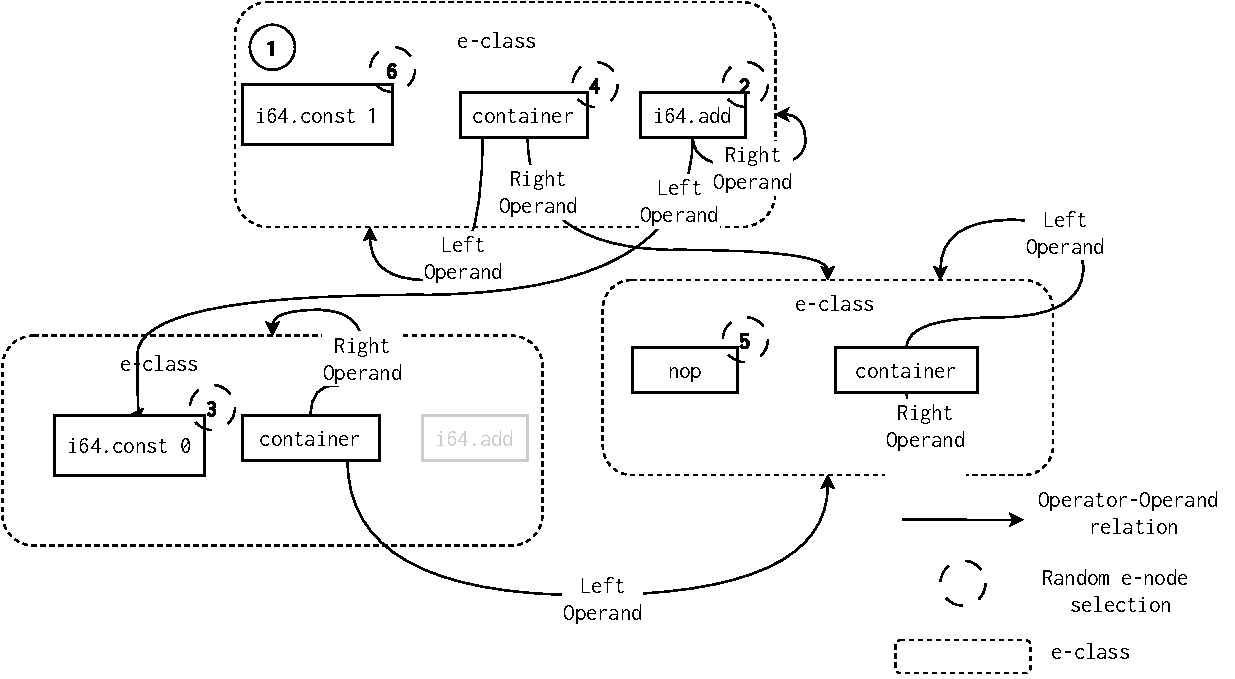
\includegraphics[width=1.0\linewidth]{figures/e-graph-traversal2.pdf}
    \caption{e-graph built for rewriting the first instruction of \autoref{example:peeporig}. }
  \label{e-graph3}
\end{figure}



Leveraging the code presented in \autoref{example:peeporig} alongside the defined rewriting rules, we build the e-graph, simplified in \autoref{e-graph3}.
In the figure, we highlight various stages of Algorithm \ref{peephole:mutator} in the context of the scenario previously described. 
The algorithm initiates at the e-class with the instruction \texttt{i64.const 1}, as seen in \autoref{example:peeporig}.
At \step{2}, it randomly selects an equivalent node within the e-class, in this instance taking the \texttt{i64.add} node, resulting: {\texttt{expr = i64.add l r}}.
As the traversal advances, it follows on the left operand of the previously chosen node, settling on the \texttt{i64.const 0} node within the same e-class \step{3}.
Then, the right operand of the \texttt{i64.add} node is choosen, selecting the \texttt{container} \step{4} operator yielding:
{\texttt{expr = i64.or (i64.const 0 container ( r nop ))}}.
The algorithm chooses the right operand of the \texttt{container} \step{5}, which correlates to the initial instruction e-node highlighted in \step{6}, culminating in the final expression:
{\texttt{expr = i64.or (i64.const 0 container( i64.const 1 nop))\ i64.const 1}}.
As we proceed to the encoding phases, the \texttt{container} operator is ignored as a real Wasm instruction, finally resulting in the program in \autoref{example:peepapplied}.

Notice that, within the e-graph showcased in \autoref{e-graph3}, the container node maintains equivalence across all e-classes. 
Consequently, increasing the depth parameter in \autoref{peephole:mutator} would potentially escalate the number of viable variants infinitely.

%s\todo{Augment this last paragraph.}


\begin{tcolorbox}[title=Contribution paper and artifact,boxrule=1pt,arc=.2em,boxsep=1.0mm]
  \tool is fully presented in Cabrera-Arteaga \etal "WASM-MUTATE: Fast and Effective Binary Diversification for WebAssembly"
 \url{https://arxiv.org/pdf/2309.07638.pdf}.
  \\\\
  \tool is available at \url{https://github.com/bytecodealliance/wasm-tools/tree/main/crates/wasm-mutate} as a contribution to the bytecodealliance organization \toolcite{https://bytecodealliance.org/}.
\end{tcolorbox}